In this chapter, we test the capabilities of  \demo{} as a framewor for
evalutating pub/sub systems. We extend the evaluation of PolderCast and
Scribe found in~\cite{Setty:2012} on a set of topology metrics. These
metrics are afforded to us for ``free'' by the Gephi framework through
the Statistics API included in the \emph{Gephi Toolkit}.

\section{\demo as a Framework for Evaluating Pub/Sub Systems}
\label{sec:viz_eval}

Although the plots seen in Chapter~\ref{ch:vizpub} are easy to produce
in Gephi, they are not very flexible. For example, it would be useful to
be able to superimpose two plots on top of each other in order to
effectively compare them. Therefore, in addition to outputting a \gexf
file which can be used to produce visualizations and plots in Gephi, The
collector is also able to generate \csv files which can be used to plot
a time series of metrics such as degree, clustering coefficient and
centralities. Each time point in the time series will represent a
\emph{Reporter Interval}. Although the Data Laboratory component in
Gephi is able to output such \csv files, it is much more convenient to
output them directly from the Collector, as opening the Gephi GUI-client
for the sole purpose of producing such files manually is more time
consuming, especially on older hardware, or machines without a dedicated
graphics card. The Collector is able to do this trough the Gephi
Toolkit, which provides an API for the major components of Gephi. Which
overlay properties to output is configurable in the Collector.
Currently, the supported metrics that can be exported to \csv files by
the Collector include:

\begin{itemize}
    \item Undirected Degree
    \item In-Degree
    \item Out-Degree
    \item Clustering Coefficient
    \item Betweenness Centrality
    \item Closeness Centrality
    \item Eccentricity Centrality
    \item Topic Diameter
    \item Size of Network
\end{itemize}

This grants researchers and developers of pub/sub protocols who wish to evaluate
the system in question immediate access to several metrics. They do not need to
reimplement algorithms for the metric calculations themselves. All that is
required is to implement the \emph{reporter interface}.

The plots produced aim at resembling the plots produced by the
Statistics Component in Gephi. However, due to using an external tool
for plotting, we can superimpose several plots on top of each other, as
well as adjust the format and layout of the plots. Also, it should be
noted that the output file format of the Gephi plots are non-vector
image files, which is not suitable for printing. The ability choose the
image format of the plots is another benefit over using the
standard plot output of Gephi.

\section{Experimental Restrictions}

As our implementation of \demo{} still is an early prototype.

\section{Experimental Setup}

We run PolderCast and Scribe in PeerNet using the simulation mode. The
Simulations consists of 1000 PeerNet cycles as well as 1000 reporter
intervals. We use workloads both from Facebook~\cite{} and
Twitter~\cite{} in order to model subscriptions. As mentioned in
Chapter~\ref{ch:vizpub}, the Facebook data trace include 3 million user
profiles along with 28.3 million friend relations. The Twitter dataset
consists of 41.7 million distinct users and 1.47 billion
follow/followed relations.

The social relations in Facebook are reciprocal, which leads us to model
bidirectional subscriptions. More specifically, a Facebook user is
modeled as a topic. The friends list of the particular user profile
constitutes its subscription list. All of the entries in this list will
include the original user in their own lists of subscriptions.
Relationships in Twitter however, are unidirectional. When using the
Twitter trace, users are also modeled as topics, but here the list of
subscriptions are formed on the basis of the ``following'' list of the
particular  user profile. The entries in this list are not required to
follow back, therefore subscriptions are also unidirectional.

Churn is based on the Skype super-peer trace from~\cite{}, tracing 4000
nodes for 4 weeks, tracking their joining and leaving timestamps. We
scale churn to include the first day of this trace in order to not
introduce a churn rate which is unrealistically high. For latency
between node pairs, we use the King dataset found in~cite{}.


\section{Results}

\subsection{Degree}

% \begin{figure}[H]
%     \centering
%     % GNUPLOT: LaTeX picture with Postscript
\begingroup
  \makeatletter
  \providecommand\color[2][]{%
    \GenericError{(gnuplot) \space\space\space\@spaces}{%
      Package color not loaded in conjunction with
      terminal option `colourtext'%
    }{See the gnuplot documentation for explanation.%
    }{Either use 'blacktext' in gnuplot or load the package
      color.sty in LaTeX.}%
    \renewcommand\color[2][]{}%
  }%
  \providecommand\includegraphics[2][]{%
    \GenericError{(gnuplot) \space\space\space\@spaces}{%
      Package graphicx or graphics not loaded%
    }{See the gnuplot documentation for explanation.%
    }{The gnuplot epslatex terminal needs graphicx.sty or graphics.sty.}%
    \renewcommand\includegraphics[2][]{}%
  }%
  \providecommand\rotatebox[2]{#2}%
  \@ifundefined{ifGPcolor}{%
    \newif\ifGPcolor
    \GPcolortrue
  }{}%
  \@ifundefined{ifGPblacktext}{%
    \newif\ifGPblacktext
    \GPblacktexttrue
  }{}%
  % define a \g@addto@macro without @ in the name:
  \let\gplgaddtomacro\g@addto@macro
  % define empty templates for all commands taking text:
  \gdef\gplbacktext{}%
  \gdef\gplfronttext{}%
  \makeatother
  \ifGPblacktext
    % no textcolor at all
    \def\colorrgb#1{}%
    \def\colorgray#1{}%
  \else
    % gray or color?
    \ifGPcolor
      \def\colorrgb#1{\color[rgb]{#1}}%
      \def\colorgray#1{\color[gray]{#1}}%
      \expandafter\def\csname LTw\endcsname{\color{white}}%
      \expandafter\def\csname LTb\endcsname{\color{black}}%
      \expandafter\def\csname LTa\endcsname{\color{black}}%
      \expandafter\def\csname LT0\endcsname{\color[rgb]{1,0,0}}%
      \expandafter\def\csname LT1\endcsname{\color[rgb]{0,1,0}}%
      \expandafter\def\csname LT2\endcsname{\color[rgb]{0,0,1}}%
      \expandafter\def\csname LT3\endcsname{\color[rgb]{1,0,1}}%
      \expandafter\def\csname LT4\endcsname{\color[rgb]{0,1,1}}%
      \expandafter\def\csname LT5\endcsname{\color[rgb]{1,1,0}}%
      \expandafter\def\csname LT6\endcsname{\color[rgb]{0,0,0}}%
      \expandafter\def\csname LT7\endcsname{\color[rgb]{1,0.3,0}}%
      \expandafter\def\csname LT8\endcsname{\color[rgb]{0.5,0.5,0.5}}%
    \else
      % gray
      \def\colorrgb#1{\color{black}}%
      \def\colorgray#1{\color[gray]{#1}}%
      \expandafter\def\csname LTw\endcsname{\color{white}}%
      \expandafter\def\csname LTb\endcsname{\color{black}}%
      \expandafter\def\csname LTa\endcsname{\color{black}}%
      \expandafter\def\csname LT0\endcsname{\color{black}}%
      \expandafter\def\csname LT1\endcsname{\color{black}}%
      \expandafter\def\csname LT2\endcsname{\color{black}}%
      \expandafter\def\csname LT3\endcsname{\color{black}}%
      \expandafter\def\csname LT4\endcsname{\color{black}}%
      \expandafter\def\csname LT5\endcsname{\color{black}}%
      \expandafter\def\csname LT6\endcsname{\color{black}}%
      \expandafter\def\csname LT7\endcsname{\color{black}}%
      \expandafter\def\csname LT8\endcsname{\color{black}}%
    \fi
  \fi
  \setlength{\unitlength}{0.0500bp}%
  \begin{picture}(7200.00,5040.00)%
    \gplgaddtomacro\gplbacktext{%
      \csname LTb\endcsname%
      \put(946,704){\makebox(0,0)[r]{\strut{} 0}}%
      \put(946,1254){\makebox(0,0)[r]{\strut{} 50}}%
      \put(946,1804){\makebox(0,0)[r]{\strut{} 100}}%
      \put(946,2355){\makebox(0,0)[r]{\strut{} 150}}%
      \put(946,2905){\makebox(0,0)[r]{\strut{} 200}}%
      \put(946,3455){\makebox(0,0)[r]{\strut{} 250}}%
      \put(1078,484){\makebox(0,0){\strut{} 0}}%
      \put(1536,484){\makebox(0,0){\strut{} 100}}%
      \put(1994,484){\makebox(0,0){\strut{} 200}}%
      \put(2452,484){\makebox(0,0){\strut{} 300}}%
      \put(2910,484){\makebox(0,0){\strut{} 400}}%
      \put(3369,484){\makebox(0,0){\strut{} 500}}%
      \put(3827,484){\makebox(0,0){\strut{} 600}}%
      \put(4285,484){\makebox(0,0){\strut{} 700}}%
      \put(4743,484){\makebox(0,0){\strut{} 800}}%
      \put(5201,484){\makebox(0,0){\strut{} 900}}%
      \put(5659,484){\makebox(0,0){\strut{} 1000}}%
      \put(5791,704){\makebox(0,0)[l]{\strut{} 0}}%
      \put(5791,979){\makebox(0,0)[l]{\strut{} 100}}%
      \put(5791,1254){\makebox(0,0)[l]{\strut{} 200}}%
      \put(5791,1529){\makebox(0,0)[l]{\strut{} 300}}%
      \put(5791,1804){\makebox(0,0)[l]{\strut{} 400}}%
      \put(5791,2080){\makebox(0,0)[l]{\strut{} 500}}%
      \put(5791,2355){\makebox(0,0)[l]{\strut{} 600}}%
      \put(5791,2630){\makebox(0,0)[l]{\strut{} 700}}%
      \put(5791,2905){\makebox(0,0)[l]{\strut{} 800}}%
      \put(5791,3180){\makebox(0,0)[l]{\strut{} 900}}%
      \put(5791,3455){\makebox(0,0)[l]{\strut{} 1000}}%
      \put(176,2079){\rotatebox{-270}{\makebox(0,0){\strut{}Degree}}}%
      \put(6692,2079){\rotatebox{-270}{\makebox(0,0){\strut{}Network Size}}}%
      \put(3368,154){\makebox(0,0){\strut{}Reporter Intervals}}%
    }%
    \gplgaddtomacro\gplfronttext{%
      \csname LTb\endcsname%
      \put(4804,4867){\makebox(0,0)[r]{\strut{}PolderCast (Facebook)}}%
      \csname LTb\endcsname%
      \put(4804,4647){\makebox(0,0)[r]{\strut{}PolderCast (Twitter)}}%
      \csname LTb\endcsname%
      \put(4804,4427){\makebox(0,0)[r]{\strut{}Scribe (Facebook)}}%
      \csname LTb\endcsname%
      \put(4804,4207){\makebox(0,0)[r]{\strut{}Scribe (Twitter)}}%
      \csname LTb\endcsname%
      \put(4804,3987){\makebox(0,0)[r]{\strut{}Network Size}}%
    }%
    \gplbacktext
    \put(0,0){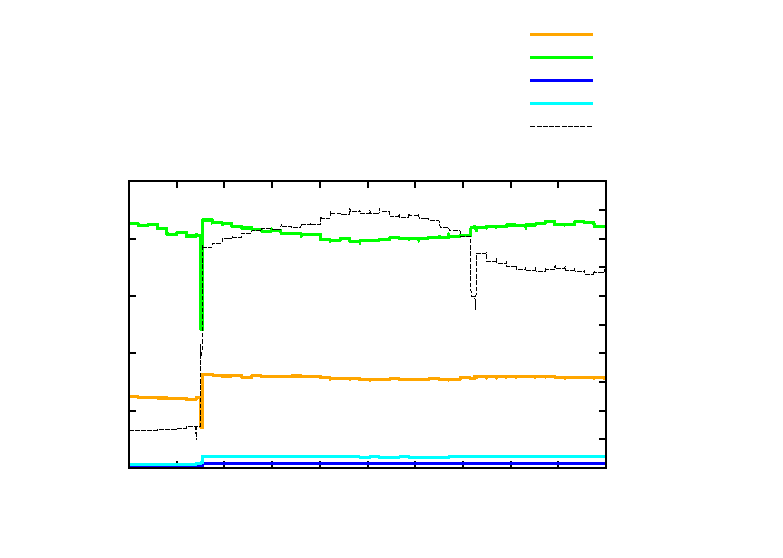
\includegraphics{eval_degree}}%
    \gplfronttext
  \end{picture}%
\endgroup

%     \caption{Avg. Undirected degree of PolderCast and Scribe}
%     \label{fig:eval_degree}
% \end{figure}

% \begin{figure}[H]
%     \centering
%     % GNUPLOT: LaTeX picture with Postscript
\begingroup
  \makeatletter
  \providecommand\color[2][]{%
    \GenericError{(gnuplot) \space\space\space\@spaces}{%
      Package color not loaded in conjunction with
      terminal option `colourtext'%
    }{See the gnuplot documentation for explanation.%
    }{Either use 'blacktext' in gnuplot or load the package
      color.sty in LaTeX.}%
    \renewcommand\color[2][]{}%
  }%
  \providecommand\includegraphics[2][]{%
    \GenericError{(gnuplot) \space\space\space\@spaces}{%
      Package graphicx or graphics not loaded%
    }{See the gnuplot documentation for explanation.%
    }{The gnuplot epslatex terminal needs graphicx.sty or graphics.sty.}%
    \renewcommand\includegraphics[2][]{}%
  }%
  \providecommand\rotatebox[2]{#2}%
  \@ifundefined{ifGPcolor}{%
    \newif\ifGPcolor
    \GPcolortrue
  }{}%
  \@ifundefined{ifGPblacktext}{%
    \newif\ifGPblacktext
    \GPblacktexttrue
  }{}%
  % define a \g@addto@macro without @ in the name:
  \let\gplgaddtomacro\g@addto@macro
  % define empty templates for all commands taking text:
  \gdef\gplbacktext{}%
  \gdef\gplfronttext{}%
  \makeatother
  \ifGPblacktext
    % no textcolor at all
    \def\colorrgb#1{}%
    \def\colorgray#1{}%
  \else
    % gray or color?
    \ifGPcolor
      \def\colorrgb#1{\color[rgb]{#1}}%
      \def\colorgray#1{\color[gray]{#1}}%
      \expandafter\def\csname LTw\endcsname{\color{white}}%
      \expandafter\def\csname LTb\endcsname{\color{black}}%
      \expandafter\def\csname LTa\endcsname{\color{black}}%
      \expandafter\def\csname LT0\endcsname{\color[rgb]{1,0,0}}%
      \expandafter\def\csname LT1\endcsname{\color[rgb]{0,1,0}}%
      \expandafter\def\csname LT2\endcsname{\color[rgb]{0,0,1}}%
      \expandafter\def\csname LT3\endcsname{\color[rgb]{1,0,1}}%
      \expandafter\def\csname LT4\endcsname{\color[rgb]{0,1,1}}%
      \expandafter\def\csname LT5\endcsname{\color[rgb]{1,1,0}}%
      \expandafter\def\csname LT6\endcsname{\color[rgb]{0,0,0}}%
      \expandafter\def\csname LT7\endcsname{\color[rgb]{1,0.3,0}}%
      \expandafter\def\csname LT8\endcsname{\color[rgb]{0.5,0.5,0.5}}%
    \else
      % gray
      \def\colorrgb#1{\color{black}}%
      \def\colorgray#1{\color[gray]{#1}}%
      \expandafter\def\csname LTw\endcsname{\color{white}}%
      \expandafter\def\csname LTb\endcsname{\color{black}}%
      \expandafter\def\csname LTa\endcsname{\color{black}}%
      \expandafter\def\csname LT0\endcsname{\color{black}}%
      \expandafter\def\csname LT1\endcsname{\color{black}}%
      \expandafter\def\csname LT2\endcsname{\color{black}}%
      \expandafter\def\csname LT3\endcsname{\color{black}}%
      \expandafter\def\csname LT4\endcsname{\color{black}}%
      \expandafter\def\csname LT5\endcsname{\color{black}}%
      \expandafter\def\csname LT6\endcsname{\color{black}}%
      \expandafter\def\csname LT7\endcsname{\color{black}}%
      \expandafter\def\csname LT8\endcsname{\color{black}}%
    \fi
  \fi
  \setlength{\unitlength}{0.0500bp}%
  \begin{picture}(7200.00,5040.00)%
    \gplgaddtomacro\gplbacktext{%
      \csname LTb\endcsname%
      \put(882,576){\makebox(0,0)[r]{\strut{} 0.1}}%
      \csname LTb\endcsname%
      \put(882,1638){\makebox(0,0)[r]{\strut{} 1}}%
      \csname LTb\endcsname%
      \put(882,2700){\makebox(0,0)[r]{\strut{} 10}}%
      \csname LTb\endcsname%
      \put(882,3761){\makebox(0,0)[r]{\strut{} 100}}%
      \csname LTb\endcsname%
      \put(882,4823){\makebox(0,0)[r]{\strut{} 1000}}%
      \csname LTb\endcsname%
      \put(990,396){\makebox(0,0){\strut{} 0}}%
      \csname LTb\endcsname%
      \put(1485,396){\makebox(0,0){\strut{} 100}}%
      \csname LTb\endcsname%
      \put(1980,396){\makebox(0,0){\strut{} 200}}%
      \csname LTb\endcsname%
      \put(2475,396){\makebox(0,0){\strut{} 300}}%
      \csname LTb\endcsname%
      \put(2970,396){\makebox(0,0){\strut{} 400}}%
      \csname LTb\endcsname%
      \put(3465,396){\makebox(0,0){\strut{} 500}}%
      \csname LTb\endcsname%
      \put(3959,396){\makebox(0,0){\strut{} 600}}%
      \csname LTb\endcsname%
      \put(4454,396){\makebox(0,0){\strut{} 700}}%
      \csname LTb\endcsname%
      \put(4949,396){\makebox(0,0){\strut{} 800}}%
      \csname LTb\endcsname%
      \put(5444,396){\makebox(0,0){\strut{} 900}}%
      \csname LTb\endcsname%
      \put(5939,396){\makebox(0,0){\strut{} 1000}}%
      \put(6047,576){\makebox(0,0)[l]{\strut{} 0}}%
      \put(6047,1001){\makebox(0,0)[l]{\strut{} 100}}%
      \put(6047,1425){\makebox(0,0)[l]{\strut{} 200}}%
      \put(6047,1850){\makebox(0,0)[l]{\strut{} 300}}%
      \put(6047,2275){\makebox(0,0)[l]{\strut{} 400}}%
      \put(6047,2700){\makebox(0,0)[l]{\strut{} 500}}%
      \put(6047,3124){\makebox(0,0)[l]{\strut{} 600}}%
      \put(6047,3549){\makebox(0,0)[l]{\strut{} 700}}%
      \put(6047,3974){\makebox(0,0)[l]{\strut{} 800}}%
      \put(6047,4398){\makebox(0,0)[l]{\strut{} 900}}%
      \put(6047,4823){\makebox(0,0)[l]{\strut{} 1000}}%
      \put(144,2699){\rotatebox{-270}{\makebox(0,0){\strut{}In-degree}}}%
      \put(6784,2699){\rotatebox{-270}{\makebox(0,0){\strut{}Network Size}}}%
      \put(3464,126){\makebox(0,0){\strut{}Reporter Intervals}}%
    }%
    \gplgaddtomacro\gplfronttext{%
      \csname LTb\endcsname%
      \put(5120,1449){\makebox(0,0)[r]{\strut{}PolderCast (Facebook)}}%
      \csname LTb\endcsname%
      \put(5120,1269){\makebox(0,0)[r]{\strut{}PolderCast (Twitter)}}%
      \csname LTb\endcsname%
      \put(5120,1089){\makebox(0,0)[r]{\strut{}Scribe (Facebook)}}%
      \csname LTb\endcsname%
      \put(5120,909){\makebox(0,0)[r]{\strut{}Scribe (Twitter)}}%
      \csname LTb\endcsname%
      \put(5120,729){\makebox(0,0)[r]{\strut{}Network Size}}%
    }%
    \gplbacktext
    \put(0,0){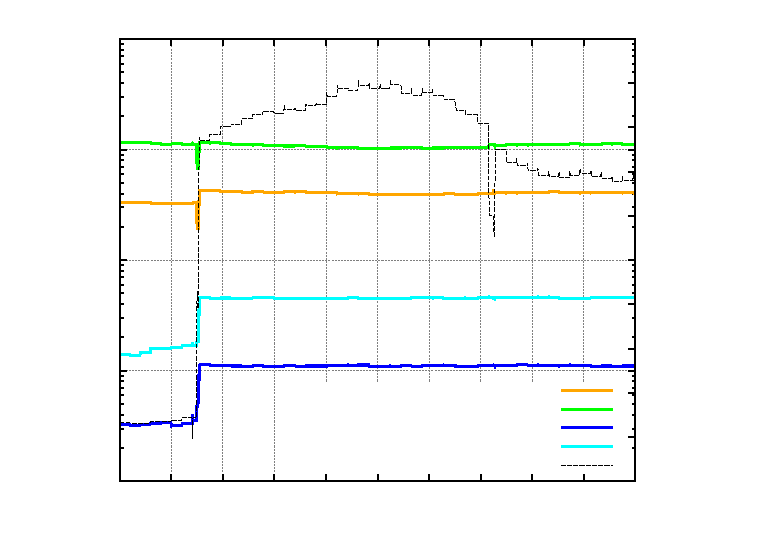
\includegraphics{eval_indegree}}%
    \gplfronttext
  \end{picture}%
\endgroup

%     \caption{Avg. In-Degree of PolderCast and Scribe}
%     \label{fig:eval_indegree}
% \end{figure}

\begin{figure}[H]
    \centering
    \subfigure[Avg. In-Degree]{
        % GNUPLOT: LaTeX picture with Postscript
\begingroup
  \makeatletter
  \providecommand\color[2][]{%
    \GenericError{(gnuplot) \space\space\space\@spaces}{%
      Package color not loaded in conjunction with
      terminal option `colourtext'%
    }{See the gnuplot documentation for explanation.%
    }{Either use 'blacktext' in gnuplot or load the package
      color.sty in LaTeX.}%
    \renewcommand\color[2][]{}%
  }%
  \providecommand\includegraphics[2][]{%
    \GenericError{(gnuplot) \space\space\space\@spaces}{%
      Package graphicx or graphics not loaded%
    }{See the gnuplot documentation for explanation.%
    }{The gnuplot epslatex terminal needs graphicx.sty or graphics.sty.}%
    \renewcommand\includegraphics[2][]{}%
  }%
  \providecommand\rotatebox[2]{#2}%
  \@ifundefined{ifGPcolor}{%
    \newif\ifGPcolor
    \GPcolortrue
  }{}%
  \@ifundefined{ifGPblacktext}{%
    \newif\ifGPblacktext
    \GPblacktexttrue
  }{}%
  % define a \g@addto@macro without @ in the name:
  \let\gplgaddtomacro\g@addto@macro
  % define empty templates for all commands taking text:
  \gdef\gplbacktext{}%
  \gdef\gplfronttext{}%
  \makeatother
  \ifGPblacktext
    % no textcolor at all
    \def\colorrgb#1{}%
    \def\colorgray#1{}%
  \else
    % gray or color?
    \ifGPcolor
      \def\colorrgb#1{\color[rgb]{#1}}%
      \def\colorgray#1{\color[gray]{#1}}%
      \expandafter\def\csname LTw\endcsname{\color{white}}%
      \expandafter\def\csname LTb\endcsname{\color{black}}%
      \expandafter\def\csname LTa\endcsname{\color{black}}%
      \expandafter\def\csname LT0\endcsname{\color[rgb]{1,0,0}}%
      \expandafter\def\csname LT1\endcsname{\color[rgb]{0,1,0}}%
      \expandafter\def\csname LT2\endcsname{\color[rgb]{0,0,1}}%
      \expandafter\def\csname LT3\endcsname{\color[rgb]{1,0,1}}%
      \expandafter\def\csname LT4\endcsname{\color[rgb]{0,1,1}}%
      \expandafter\def\csname LT5\endcsname{\color[rgb]{1,1,0}}%
      \expandafter\def\csname LT6\endcsname{\color[rgb]{0,0,0}}%
      \expandafter\def\csname LT7\endcsname{\color[rgb]{1,0.3,0}}%
      \expandafter\def\csname LT8\endcsname{\color[rgb]{0.5,0.5,0.5}}%
    \else
      % gray
      \def\colorrgb#1{\color{black}}%
      \def\colorgray#1{\color[gray]{#1}}%
      \expandafter\def\csname LTw\endcsname{\color{white}}%
      \expandafter\def\csname LTb\endcsname{\color{black}}%
      \expandafter\def\csname LTa\endcsname{\color{black}}%
      \expandafter\def\csname LT0\endcsname{\color{black}}%
      \expandafter\def\csname LT1\endcsname{\color{black}}%
      \expandafter\def\csname LT2\endcsname{\color{black}}%
      \expandafter\def\csname LT3\endcsname{\color{black}}%
      \expandafter\def\csname LT4\endcsname{\color{black}}%
      \expandafter\def\csname LT5\endcsname{\color{black}}%
      \expandafter\def\csname LT6\endcsname{\color{black}}%
      \expandafter\def\csname LT7\endcsname{\color{black}}%
      \expandafter\def\csname LT8\endcsname{\color{black}}%
    \fi
  \fi
  \setlength{\unitlength}{0.0500bp}%
  \begin{picture}(7200.00,5040.00)%
    \gplgaddtomacro\gplbacktext{%
      \csname LTb\endcsname%
      \put(882,576){\makebox(0,0)[r]{\strut{} 0.1}}%
      \csname LTb\endcsname%
      \put(882,1638){\makebox(0,0)[r]{\strut{} 1}}%
      \csname LTb\endcsname%
      \put(882,2700){\makebox(0,0)[r]{\strut{} 10}}%
      \csname LTb\endcsname%
      \put(882,3761){\makebox(0,0)[r]{\strut{} 100}}%
      \csname LTb\endcsname%
      \put(882,4823){\makebox(0,0)[r]{\strut{} 1000}}%
      \csname LTb\endcsname%
      \put(990,396){\makebox(0,0){\strut{} 0}}%
      \csname LTb\endcsname%
      \put(1485,396){\makebox(0,0){\strut{} 100}}%
      \csname LTb\endcsname%
      \put(1980,396){\makebox(0,0){\strut{} 200}}%
      \csname LTb\endcsname%
      \put(2475,396){\makebox(0,0){\strut{} 300}}%
      \csname LTb\endcsname%
      \put(2970,396){\makebox(0,0){\strut{} 400}}%
      \csname LTb\endcsname%
      \put(3465,396){\makebox(0,0){\strut{} 500}}%
      \csname LTb\endcsname%
      \put(3959,396){\makebox(0,0){\strut{} 600}}%
      \csname LTb\endcsname%
      \put(4454,396){\makebox(0,0){\strut{} 700}}%
      \csname LTb\endcsname%
      \put(4949,396){\makebox(0,0){\strut{} 800}}%
      \csname LTb\endcsname%
      \put(5444,396){\makebox(0,0){\strut{} 900}}%
      \csname LTb\endcsname%
      \put(5939,396){\makebox(0,0){\strut{} 1000}}%
      \put(6047,576){\makebox(0,0)[l]{\strut{} 0}}%
      \put(6047,1001){\makebox(0,0)[l]{\strut{} 100}}%
      \put(6047,1425){\makebox(0,0)[l]{\strut{} 200}}%
      \put(6047,1850){\makebox(0,0)[l]{\strut{} 300}}%
      \put(6047,2275){\makebox(0,0)[l]{\strut{} 400}}%
      \put(6047,2700){\makebox(0,0)[l]{\strut{} 500}}%
      \put(6047,3124){\makebox(0,0)[l]{\strut{} 600}}%
      \put(6047,3549){\makebox(0,0)[l]{\strut{} 700}}%
      \put(6047,3974){\makebox(0,0)[l]{\strut{} 800}}%
      \put(6047,4398){\makebox(0,0)[l]{\strut{} 900}}%
      \put(6047,4823){\makebox(0,0)[l]{\strut{} 1000}}%
      \put(144,2699){\rotatebox{-270}{\makebox(0,0){\strut{}In-degree}}}%
      \put(6784,2699){\rotatebox{-270}{\makebox(0,0){\strut{}Network Size}}}%
      \put(3464,126){\makebox(0,0){\strut{}Reporter Intervals}}%
    }%
    \gplgaddtomacro\gplfronttext{%
      \csname LTb\endcsname%
      \put(5120,1449){\makebox(0,0)[r]{\strut{}PolderCast (Facebook)}}%
      \csname LTb\endcsname%
      \put(5120,1269){\makebox(0,0)[r]{\strut{}PolderCast (Twitter)}}%
      \csname LTb\endcsname%
      \put(5120,1089){\makebox(0,0)[r]{\strut{}Scribe (Facebook)}}%
      \csname LTb\endcsname%
      \put(5120,909){\makebox(0,0)[r]{\strut{}Scribe (Twitter)}}%
      \csname LTb\endcsname%
      \put(5120,729){\makebox(0,0)[r]{\strut{}Network Size}}%
    }%
    \gplbacktext
    \put(0,0){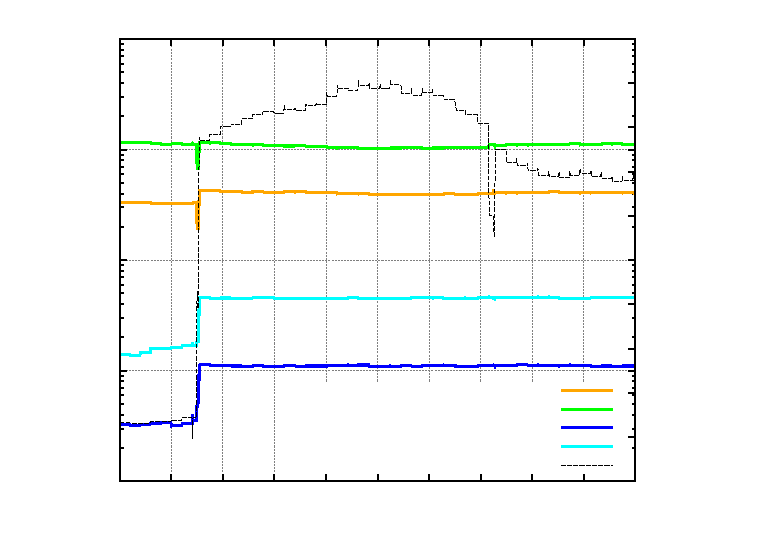
\includegraphics{eval_indegree}}%
    \gplfronttext
  \end{picture}%
\endgroup

    }
    \subfigure[Avg. Out-Degree]{
        % GNUPLOT: LaTeX picture with Postscript
\begingroup
  \makeatletter
  \providecommand\color[2][]{%
    \GenericError{(gnuplot) \space\space\space\@spaces}{%
      Package color not loaded in conjunction with
      terminal option `colourtext'%
    }{See the gnuplot documentation for explanation.%
    }{Either use 'blacktext' in gnuplot or load the package
      color.sty in LaTeX.}%
    \renewcommand\color[2][]{}%
  }%
  \providecommand\includegraphics[2][]{%
    \GenericError{(gnuplot) \space\space\space\@spaces}{%
      Package graphicx or graphics not loaded%
    }{See the gnuplot documentation for explanation.%
    }{The gnuplot epslatex terminal needs graphicx.sty or graphics.sty.}%
    \renewcommand\includegraphics[2][]{}%
  }%
  \providecommand\rotatebox[2]{#2}%
  \@ifundefined{ifGPcolor}{%
    \newif\ifGPcolor
    \GPcolortrue
  }{}%
  \@ifundefined{ifGPblacktext}{%
    \newif\ifGPblacktext
    \GPblacktexttrue
  }{}%
  % define a \g@addto@macro without @ in the name:
  \let\gplgaddtomacro\g@addto@macro
  % define empty templates for all commands taking text:
  \gdef\gplbacktext{}%
  \gdef\gplfronttext{}%
  \makeatother
  \ifGPblacktext
    % no textcolor at all
    \def\colorrgb#1{}%
    \def\colorgray#1{}%
  \else
    % gray or color?
    \ifGPcolor
      \def\colorrgb#1{\color[rgb]{#1}}%
      \def\colorgray#1{\color[gray]{#1}}%
      \expandafter\def\csname LTw\endcsname{\color{white}}%
      \expandafter\def\csname LTb\endcsname{\color{black}}%
      \expandafter\def\csname LTa\endcsname{\color{black}}%
      \expandafter\def\csname LT0\endcsname{\color[rgb]{1,0,0}}%
      \expandafter\def\csname LT1\endcsname{\color[rgb]{0,1,0}}%
      \expandafter\def\csname LT2\endcsname{\color[rgb]{0,0,1}}%
      \expandafter\def\csname LT3\endcsname{\color[rgb]{1,0,1}}%
      \expandafter\def\csname LT4\endcsname{\color[rgb]{0,1,1}}%
      \expandafter\def\csname LT5\endcsname{\color[rgb]{1,1,0}}%
      \expandafter\def\csname LT6\endcsname{\color[rgb]{0,0,0}}%
      \expandafter\def\csname LT7\endcsname{\color[rgb]{1,0.3,0}}%
      \expandafter\def\csname LT8\endcsname{\color[rgb]{0.5,0.5,0.5}}%
    \else
      % gray
      \def\colorrgb#1{\color{black}}%
      \def\colorgray#1{\color[gray]{#1}}%
      \expandafter\def\csname LTw\endcsname{\color{white}}%
      \expandafter\def\csname LTb\endcsname{\color{black}}%
      \expandafter\def\csname LTa\endcsname{\color{black}}%
      \expandafter\def\csname LT0\endcsname{\color{black}}%
      \expandafter\def\csname LT1\endcsname{\color{black}}%
      \expandafter\def\csname LT2\endcsname{\color{black}}%
      \expandafter\def\csname LT3\endcsname{\color{black}}%
      \expandafter\def\csname LT4\endcsname{\color{black}}%
      \expandafter\def\csname LT5\endcsname{\color{black}}%
      \expandafter\def\csname LT6\endcsname{\color{black}}%
      \expandafter\def\csname LT7\endcsname{\color{black}}%
      \expandafter\def\csname LT8\endcsname{\color{black}}%
    \fi
  \fi
  \setlength{\unitlength}{0.0500bp}%
  \begin{picture}(7200.00,5040.00)%
    \gplgaddtomacro\gplbacktext{%
      \csname LTb\endcsname%
      \put(882,576){\makebox(0,0)[r]{\strut{} 0.1}}%
      \csname LTb\endcsname%
      \put(882,1638){\makebox(0,0)[r]{\strut{} 1}}%
      \csname LTb\endcsname%
      \put(882,2700){\makebox(0,0)[r]{\strut{} 10}}%
      \csname LTb\endcsname%
      \put(882,3761){\makebox(0,0)[r]{\strut{} 100}}%
      \csname LTb\endcsname%
      \put(882,4823){\makebox(0,0)[r]{\strut{} 1000}}%
      \csname LTb\endcsname%
      \put(990,396){\makebox(0,0){\strut{} 0}}%
      \csname LTb\endcsname%
      \put(1485,396){\makebox(0,0){\strut{} 100}}%
      \csname LTb\endcsname%
      \put(1980,396){\makebox(0,0){\strut{} 200}}%
      \csname LTb\endcsname%
      \put(2475,396){\makebox(0,0){\strut{} 300}}%
      \csname LTb\endcsname%
      \put(2970,396){\makebox(0,0){\strut{} 400}}%
      \csname LTb\endcsname%
      \put(3465,396){\makebox(0,0){\strut{} 500}}%
      \csname LTb\endcsname%
      \put(3959,396){\makebox(0,0){\strut{} 600}}%
      \csname LTb\endcsname%
      \put(4454,396){\makebox(0,0){\strut{} 700}}%
      \csname LTb\endcsname%
      \put(4949,396){\makebox(0,0){\strut{} 800}}%
      \csname LTb\endcsname%
      \put(5444,396){\makebox(0,0){\strut{} 900}}%
      \csname LTb\endcsname%
      \put(5939,396){\makebox(0,0){\strut{} 1000}}%
      \put(6047,576){\makebox(0,0)[l]{\strut{} 0}}%
      \put(6047,1001){\makebox(0,0)[l]{\strut{} 100}}%
      \put(6047,1425){\makebox(0,0)[l]{\strut{} 200}}%
      \put(6047,1850){\makebox(0,0)[l]{\strut{} 300}}%
      \put(6047,2275){\makebox(0,0)[l]{\strut{} 400}}%
      \put(6047,2700){\makebox(0,0)[l]{\strut{} 500}}%
      \put(6047,3124){\makebox(0,0)[l]{\strut{} 600}}%
      \put(6047,3549){\makebox(0,0)[l]{\strut{} 700}}%
      \put(6047,3974){\makebox(0,0)[l]{\strut{} 800}}%
      \put(6047,4398){\makebox(0,0)[l]{\strut{} 900}}%
      \put(6047,4823){\makebox(0,0)[l]{\strut{} 1000}}%
      \put(144,2699){\rotatebox{-270}{\makebox(0,0){\strut{}Avg. Out-Degree}}}%
      \put(6784,2699){\rotatebox{-270}{\makebox(0,0){\strut{}Network Size}}}%
      \put(3464,126){\makebox(0,0){\strut{}Reporter Intervals}}%
    }%
    \gplgaddtomacro\gplfronttext{%
      \csname LTb\endcsname%
      \put(5120,1449){\makebox(0,0)[r]{\strut{}PolderCast (Facebook)}}%
      \csname LTb\endcsname%
      \put(5120,1269){\makebox(0,0)[r]{\strut{}PolderCast (Twitter)}}%
      \csname LTb\endcsname%
      \put(5120,1089){\makebox(0,0)[r]{\strut{}Scribe (Facebook)}}%
      \csname LTb\endcsname%
      \put(5120,909){\makebox(0,0)[r]{\strut{}Scribe (Twitter)}}%
      \csname LTb\endcsname%
      \put(5120,729){\makebox(0,0)[r]{\strut{}Network Size}}%
    }%
    \gplbacktext
    \put(0,0){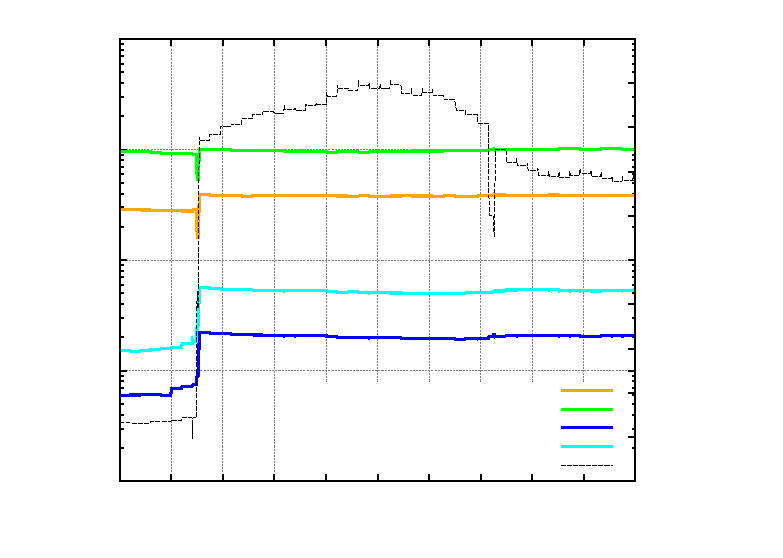
\includegraphics{eval_outdegree}}%
    \gplfronttext
  \end{picture}%
\endgroup

    }
    \caption{Avg. Directed Degrees of PolderCast and Scribe}
    \label{fig:eval_directedtdegree}
\end{figure}

\subsection{Clustering Coefficient}
\begin{figure}[H]
    \centering
    % GNUPLOT: LaTeX picture with Postscript
\begingroup
  \makeatletter
  \providecommand\color[2][]{%
    \GenericError{(gnuplot) \space\space\space\@spaces}{%
      Package color not loaded in conjunction with
      terminal option `colourtext'%
    }{See the gnuplot documentation for explanation.%
    }{Either use 'blacktext' in gnuplot or load the package
      color.sty in LaTeX.}%
    \renewcommand\color[2][]{}%
  }%
  \providecommand\includegraphics[2][]{%
    \GenericError{(gnuplot) \space\space\space\@spaces}{%
      Package graphicx or graphics not loaded%
    }{See the gnuplot documentation for explanation.%
    }{The gnuplot epslatex terminal needs graphicx.sty or graphics.sty.}%
    \renewcommand\includegraphics[2][]{}%
  }%
  \providecommand\rotatebox[2]{#2}%
  \@ifundefined{ifGPcolor}{%
    \newif\ifGPcolor
    \GPcolortrue
  }{}%
  \@ifundefined{ifGPblacktext}{%
    \newif\ifGPblacktext
    \GPblacktexttrue
  }{}%
  % define a \g@addto@macro without @ in the name:
  \let\gplgaddtomacro\g@addto@macro
  % define empty templates for all commands taking text:
  \gdef\gplbacktext{}%
  \gdef\gplfronttext{}%
  \makeatother
  \ifGPblacktext
    % no textcolor at all
    \def\colorrgb#1{}%
    \def\colorgray#1{}%
  \else
    % gray or color?
    \ifGPcolor
      \def\colorrgb#1{\color[rgb]{#1}}%
      \def\colorgray#1{\color[gray]{#1}}%
      \expandafter\def\csname LTw\endcsname{\color{white}}%
      \expandafter\def\csname LTb\endcsname{\color{black}}%
      \expandafter\def\csname LTa\endcsname{\color{black}}%
      \expandafter\def\csname LT0\endcsname{\color[rgb]{1,0,0}}%
      \expandafter\def\csname LT1\endcsname{\color[rgb]{0,1,0}}%
      \expandafter\def\csname LT2\endcsname{\color[rgb]{0,0,1}}%
      \expandafter\def\csname LT3\endcsname{\color[rgb]{1,0,1}}%
      \expandafter\def\csname LT4\endcsname{\color[rgb]{0,1,1}}%
      \expandafter\def\csname LT5\endcsname{\color[rgb]{1,1,0}}%
      \expandafter\def\csname LT6\endcsname{\color[rgb]{0,0,0}}%
      \expandafter\def\csname LT7\endcsname{\color[rgb]{1,0.3,0}}%
      \expandafter\def\csname LT8\endcsname{\color[rgb]{0.5,0.5,0.5}}%
    \else
      % gray
      \def\colorrgb#1{\color{black}}%
      \def\colorgray#1{\color[gray]{#1}}%
      \expandafter\def\csname LTw\endcsname{\color{white}}%
      \expandafter\def\csname LTb\endcsname{\color{black}}%
      \expandafter\def\csname LTa\endcsname{\color{black}}%
      \expandafter\def\csname LT0\endcsname{\color{black}}%
      \expandafter\def\csname LT1\endcsname{\color{black}}%
      \expandafter\def\csname LT2\endcsname{\color{black}}%
      \expandafter\def\csname LT3\endcsname{\color{black}}%
      \expandafter\def\csname LT4\endcsname{\color{black}}%
      \expandafter\def\csname LT5\endcsname{\color{black}}%
      \expandafter\def\csname LT6\endcsname{\color{black}}%
      \expandafter\def\csname LT7\endcsname{\color{black}}%
      \expandafter\def\csname LT8\endcsname{\color{black}}%
    \fi
  \fi
  \setlength{\unitlength}{0.0500bp}%
  \begin{picture}(7200.00,5040.00)%
    \gplgaddtomacro\gplbacktext{%
      \csname LTb\endcsname%
      \put(1342,704){\makebox(0,0)[r]{\strut{} 0.0001}}%
      \csname LTb\endcsname%
      \put(1342,1722){\makebox(0,0)[r]{\strut{} 0.001}}%
      \csname LTb\endcsname%
      \put(1342,2740){\makebox(0,0)[r]{\strut{} 0.01}}%
      \csname LTb\endcsname%
      \put(1342,3757){\makebox(0,0)[r]{\strut{} 0.1}}%
      \csname LTb\endcsname%
      \put(1342,4775){\makebox(0,0)[r]{\strut{} 1}}%
      \csname LTb\endcsname%
      \put(1474,484){\makebox(0,0){\strut{} 0}}%
      \csname LTb\endcsname%
      \put(1893,484){\makebox(0,0){\strut{} 100}}%
      \csname LTb\endcsname%
      \put(2311,484){\makebox(0,0){\strut{} 200}}%
      \csname LTb\endcsname%
      \put(2730,484){\makebox(0,0){\strut{} 300}}%
      \csname LTb\endcsname%
      \put(3148,484){\makebox(0,0){\strut{} 400}}%
      \csname LTb\endcsname%
      \put(3567,484){\makebox(0,0){\strut{} 500}}%
      \csname LTb\endcsname%
      \put(3985,484){\makebox(0,0){\strut{} 600}}%
      \csname LTb\endcsname%
      \put(4404,484){\makebox(0,0){\strut{} 700}}%
      \csname LTb\endcsname%
      \put(4822,484){\makebox(0,0){\strut{} 800}}%
      \csname LTb\endcsname%
      \put(5241,484){\makebox(0,0){\strut{} 900}}%
      \csname LTb\endcsname%
      \put(5659,484){\makebox(0,0){\strut{} 1000}}%
      \put(5791,704){\makebox(0,0)[l]{\strut{} 0}}%
      \put(5791,1111){\makebox(0,0)[l]{\strut{} 100}}%
      \put(5791,1518){\makebox(0,0)[l]{\strut{} 200}}%
      \put(5791,1925){\makebox(0,0)[l]{\strut{} 300}}%
      \put(5791,2332){\makebox(0,0)[l]{\strut{} 400}}%
      \put(5791,2740){\makebox(0,0)[l]{\strut{} 500}}%
      \put(5791,3147){\makebox(0,0)[l]{\strut{} 600}}%
      \put(5791,3554){\makebox(0,0)[l]{\strut{} 700}}%
      \put(5791,3961){\makebox(0,0)[l]{\strut{} 800}}%
      \put(5791,4368){\makebox(0,0)[l]{\strut{} 900}}%
      \put(5791,4775){\makebox(0,0)[l]{\strut{} 1000}}%
      \put(176,2739){\rotatebox{-270}{\makebox(0,0){\strut{}Avg. Clustering Coefficient}}}%
      \put(6692,2739){\rotatebox{-270}{\makebox(0,0){\strut{}Network Size}}}%
      \put(3566,154){\makebox(0,0){\strut{}Reporter Intervals}}%
    }%
    \gplgaddtomacro\gplfronttext{%
      \csname LTb\endcsname%
      \put(4672,1757){\makebox(0,0)[r]{\strut{}PolderCast (Facebook)}}%
      \csname LTb\endcsname%
      \put(4672,1537){\makebox(0,0)[r]{\strut{}PolderCast (Twitter)}}%
      \csname LTb\endcsname%
      \put(4672,1317){\makebox(0,0)[r]{\strut{}Scribe (Facebook)}}%
      \csname LTb\endcsname%
      \put(4672,1097){\makebox(0,0)[r]{\strut{}Scribe (Twitter)}}%
      \csname LTb\endcsname%
      \put(4672,877){\makebox(0,0)[r]{\strut{}Network Size}}%
    }%
    \gplbacktext
    \put(0,0){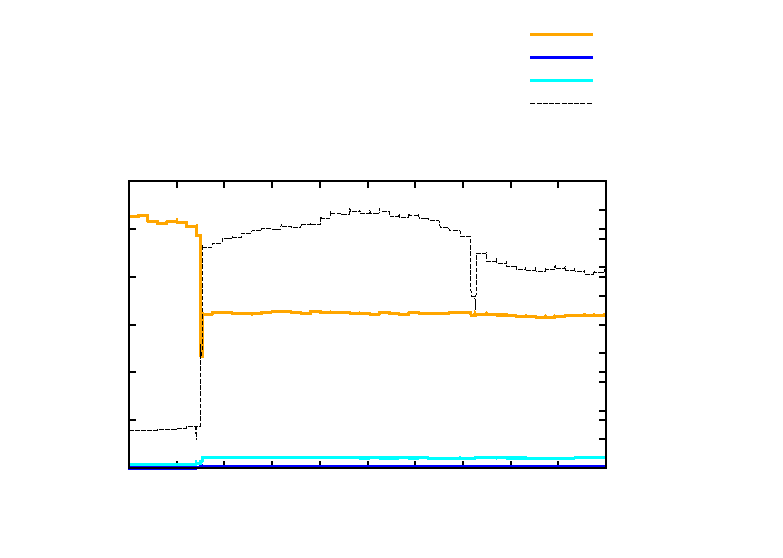
\includegraphics{eval_cc}}%
    \gplfronttext
  \end{picture}%
\endgroup

    \caption{Avg. Clustering Coefficient of PolderCast and Scribe}
    \label{fig:eval_cc}
\end{figure}

\subsection{Centralities}

% \begin{figure}[H]
%     \centering
%     % GNUPLOT: LaTeX picture with Postscript
\begingroup
  \makeatletter
  \providecommand\color[2][]{%
    \GenericError{(gnuplot) \space\space\space\@spaces}{%
      Package color not loaded in conjunction with
      terminal option `colourtext'%
    }{See the gnuplot documentation for explanation.%
    }{Either use 'blacktext' in gnuplot or load the package
      color.sty in LaTeX.}%
    \renewcommand\color[2][]{}%
  }%
  \providecommand\includegraphics[2][]{%
    \GenericError{(gnuplot) \space\space\space\@spaces}{%
      Package graphicx or graphics not loaded%
    }{See the gnuplot documentation for explanation.%
    }{The gnuplot epslatex terminal needs graphicx.sty or graphics.sty.}%
    \renewcommand\includegraphics[2][]{}%
  }%
  \providecommand\rotatebox[2]{#2}%
  \@ifundefined{ifGPcolor}{%
    \newif\ifGPcolor
    \GPcolortrue
  }{}%
  \@ifundefined{ifGPblacktext}{%
    \newif\ifGPblacktext
    \GPblacktexttrue
  }{}%
  % define a \g@addto@macro without @ in the name:
  \let\gplgaddtomacro\g@addto@macro
  % define empty templates for all commands taking text:
  \gdef\gplbacktext{}%
  \gdef\gplfronttext{}%
  \makeatother
  \ifGPblacktext
    % no textcolor at all
    \def\colorrgb#1{}%
    \def\colorgray#1{}%
  \else
    % gray or color?
    \ifGPcolor
      \def\colorrgb#1{\color[rgb]{#1}}%
      \def\colorgray#1{\color[gray]{#1}}%
      \expandafter\def\csname LTw\endcsname{\color{white}}%
      \expandafter\def\csname LTb\endcsname{\color{black}}%
      \expandafter\def\csname LTa\endcsname{\color{black}}%
      \expandafter\def\csname LT0\endcsname{\color[rgb]{1,0,0}}%
      \expandafter\def\csname LT1\endcsname{\color[rgb]{0,1,0}}%
      \expandafter\def\csname LT2\endcsname{\color[rgb]{0,0,1}}%
      \expandafter\def\csname LT3\endcsname{\color[rgb]{1,0,1}}%
      \expandafter\def\csname LT4\endcsname{\color[rgb]{0,1,1}}%
      \expandafter\def\csname LT5\endcsname{\color[rgb]{1,1,0}}%
      \expandafter\def\csname LT6\endcsname{\color[rgb]{0,0,0}}%
      \expandafter\def\csname LT7\endcsname{\color[rgb]{1,0.3,0}}%
      \expandafter\def\csname LT8\endcsname{\color[rgb]{0.5,0.5,0.5}}%
    \else
      % gray
      \def\colorrgb#1{\color{black}}%
      \def\colorgray#1{\color[gray]{#1}}%
      \expandafter\def\csname LTw\endcsname{\color{white}}%
      \expandafter\def\csname LTb\endcsname{\color{black}}%
      \expandafter\def\csname LTa\endcsname{\color{black}}%
      \expandafter\def\csname LT0\endcsname{\color{black}}%
      \expandafter\def\csname LT1\endcsname{\color{black}}%
      \expandafter\def\csname LT2\endcsname{\color{black}}%
      \expandafter\def\csname LT3\endcsname{\color{black}}%
      \expandafter\def\csname LT4\endcsname{\color{black}}%
      \expandafter\def\csname LT5\endcsname{\color{black}}%
      \expandafter\def\csname LT6\endcsname{\color{black}}%
      \expandafter\def\csname LT7\endcsname{\color{black}}%
      \expandafter\def\csname LT8\endcsname{\color{black}}%
    \fi
  \fi
  \setlength{\unitlength}{0.0500bp}%
  \begin{picture}(7200.00,5040.00)%
    \gplgaddtomacro\gplbacktext{%
      \csname LTb\endcsname%
      \put(1078,704){\makebox(0,0)[r]{\strut{} 0}}%
      \put(1078,1163){\makebox(0,0)[r]{\strut{} 1000}}%
      \put(1078,1621){\makebox(0,0)[r]{\strut{} 2000}}%
      \put(1078,2080){\makebox(0,0)[r]{\strut{} 3000}}%
      \put(1078,2538){\makebox(0,0)[r]{\strut{} 4000}}%
      \put(1078,2997){\makebox(0,0)[r]{\strut{} 5000}}%
      \put(1078,3455){\makebox(0,0)[r]{\strut{} 6000}}%
      \put(1210,484){\makebox(0,0){\strut{} 0}}%
      \put(1655,484){\makebox(0,0){\strut{} 100}}%
      \put(2100,484){\makebox(0,0){\strut{} 200}}%
      \put(2545,484){\makebox(0,0){\strut{} 300}}%
      \put(2990,484){\makebox(0,0){\strut{} 400}}%
      \put(3435,484){\makebox(0,0){\strut{} 500}}%
      \put(3879,484){\makebox(0,0){\strut{} 600}}%
      \put(4324,484){\makebox(0,0){\strut{} 700}}%
      \put(4769,484){\makebox(0,0){\strut{} 800}}%
      \put(5214,484){\makebox(0,0){\strut{} 900}}%
      \put(5659,484){\makebox(0,0){\strut{} 1000}}%
      \put(5791,704){\makebox(0,0)[l]{\strut{} 0}}%
      \put(5791,979){\makebox(0,0)[l]{\strut{} 100}}%
      \put(5791,1254){\makebox(0,0)[l]{\strut{} 200}}%
      \put(5791,1529){\makebox(0,0)[l]{\strut{} 300}}%
      \put(5791,1804){\makebox(0,0)[l]{\strut{} 400}}%
      \put(5791,2080){\makebox(0,0)[l]{\strut{} 500}}%
      \put(5791,2355){\makebox(0,0)[l]{\strut{} 600}}%
      \put(5791,2630){\makebox(0,0)[l]{\strut{} 700}}%
      \put(5791,2905){\makebox(0,0)[l]{\strut{} 800}}%
      \put(5791,3180){\makebox(0,0)[l]{\strut{} 900}}%
      \put(5791,3455){\makebox(0,0)[l]{\strut{} 1000}}%
      \put(176,2079){\rotatebox{-270}{\makebox(0,0){\strut{}Betweenness Centrality}}}%
      \put(6692,2079){\rotatebox{-270}{\makebox(0,0){\strut{}Network Size}}}%
      \put(3434,154){\makebox(0,0){\strut{}Reporter Intervals}}%
    }%
    \gplgaddtomacro\gplfronttext{%
      \csname LTb\endcsname%
      \put(4804,4867){\makebox(0,0)[r]{\strut{}PolderCast (Facebook)}}%
      \csname LTb\endcsname%
      \put(4804,4647){\makebox(0,0)[r]{\strut{}PolderCast (Twitter)}}%
      \csname LTb\endcsname%
      \put(4804,4427){\makebox(0,0)[r]{\strut{}Scribe (Facebook)}}%
      \csname LTb\endcsname%
      \put(4804,4207){\makebox(0,0)[r]{\strut{}Scribe (Twitter)}}%
      \csname LTb\endcsname%
      \put(4804,3987){\makebox(0,0)[r]{\strut{}Network Size}}%
    }%
    \gplbacktext
    \put(0,0){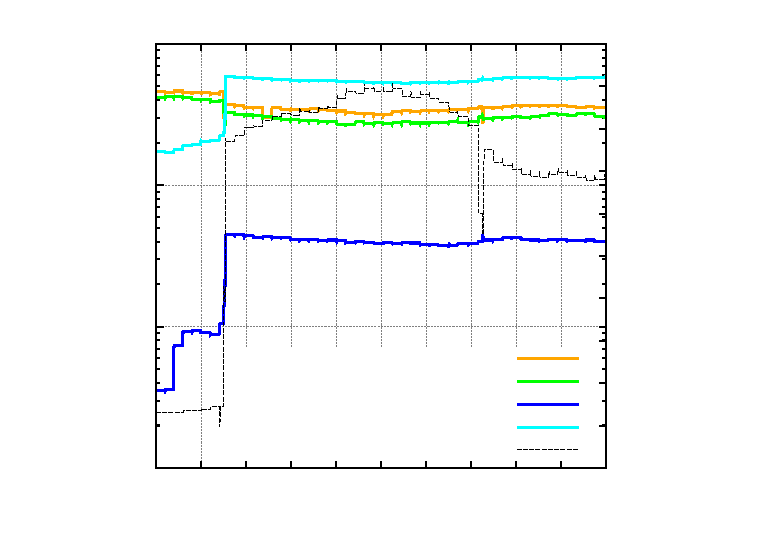
\includegraphics{eval_betweenness}}%
    \gplfronttext
  \end{picture}%
\endgroup

%     \caption{Avg. Betweenness Centrality of PolderCast and Scribe}
%     \label{fig:eval_betweenness}
% \end{figure}

% \begin{figure}[H]
%     \centering
%     % GNUPLOT: LaTeX picture with Postscript
\begingroup
  \makeatletter
  \providecommand\color[2][]{%
    \GenericError{(gnuplot) \space\space\space\@spaces}{%
      Package color not loaded in conjunction with
      terminal option `colourtext'%
    }{See the gnuplot documentation for explanation.%
    }{Either use 'blacktext' in gnuplot or load the package
      color.sty in LaTeX.}%
    \renewcommand\color[2][]{}%
  }%
  \providecommand\includegraphics[2][]{%
    \GenericError{(gnuplot) \space\space\space\@spaces}{%
      Package graphicx or graphics not loaded%
    }{See the gnuplot documentation for explanation.%
    }{The gnuplot epslatex terminal needs graphicx.sty or graphics.sty.}%
    \renewcommand\includegraphics[2][]{}%
  }%
  \providecommand\rotatebox[2]{#2}%
  \@ifundefined{ifGPcolor}{%
    \newif\ifGPcolor
    \GPcolortrue
  }{}%
  \@ifundefined{ifGPblacktext}{%
    \newif\ifGPblacktext
    \GPblacktexttrue
  }{}%
  % define a \g@addto@macro without @ in the name:
  \let\gplgaddtomacro\g@addto@macro
  % define empty templates for all commands taking text:
  \gdef\gplbacktext{}%
  \gdef\gplfronttext{}%
  \makeatother
  \ifGPblacktext
    % no textcolor at all
    \def\colorrgb#1{}%
    \def\colorgray#1{}%
  \else
    % gray or color?
    \ifGPcolor
      \def\colorrgb#1{\color[rgb]{#1}}%
      \def\colorgray#1{\color[gray]{#1}}%
      \expandafter\def\csname LTw\endcsname{\color{white}}%
      \expandafter\def\csname LTb\endcsname{\color{black}}%
      \expandafter\def\csname LTa\endcsname{\color{black}}%
      \expandafter\def\csname LT0\endcsname{\color[rgb]{1,0,0}}%
      \expandafter\def\csname LT1\endcsname{\color[rgb]{0,1,0}}%
      \expandafter\def\csname LT2\endcsname{\color[rgb]{0,0,1}}%
      \expandafter\def\csname LT3\endcsname{\color[rgb]{1,0,1}}%
      \expandafter\def\csname LT4\endcsname{\color[rgb]{0,1,1}}%
      \expandafter\def\csname LT5\endcsname{\color[rgb]{1,1,0}}%
      \expandafter\def\csname LT6\endcsname{\color[rgb]{0,0,0}}%
      \expandafter\def\csname LT7\endcsname{\color[rgb]{1,0.3,0}}%
      \expandafter\def\csname LT8\endcsname{\color[rgb]{0.5,0.5,0.5}}%
    \else
      % gray
      \def\colorrgb#1{\color{black}}%
      \def\colorgray#1{\color[gray]{#1}}%
      \expandafter\def\csname LTw\endcsname{\color{white}}%
      \expandafter\def\csname LTb\endcsname{\color{black}}%
      \expandafter\def\csname LTa\endcsname{\color{black}}%
      \expandafter\def\csname LT0\endcsname{\color{black}}%
      \expandafter\def\csname LT1\endcsname{\color{black}}%
      \expandafter\def\csname LT2\endcsname{\color{black}}%
      \expandafter\def\csname LT3\endcsname{\color{black}}%
      \expandafter\def\csname LT4\endcsname{\color{black}}%
      \expandafter\def\csname LT5\endcsname{\color{black}}%
      \expandafter\def\csname LT6\endcsname{\color{black}}%
      \expandafter\def\csname LT7\endcsname{\color{black}}%
      \expandafter\def\csname LT8\endcsname{\color{black}}%
    \fi
  \fi
  \setlength{\unitlength}{0.0500bp}%
  \begin{picture}(7200.00,5040.00)%
    \gplgaddtomacro\gplbacktext{%
      \csname LTb\endcsname%
      \put(946,704){\makebox(0,0)[r]{\strut{} 0}}%
      \csname LTb\endcsname%
      \put(946,1111){\makebox(0,0)[r]{\strut{} 0.5}}%
      \csname LTb\endcsname%
      \put(946,1518){\makebox(0,0)[r]{\strut{} 1}}%
      \csname LTb\endcsname%
      \put(946,1925){\makebox(0,0)[r]{\strut{} 1.5}}%
      \csname LTb\endcsname%
      \put(946,2332){\makebox(0,0)[r]{\strut{} 2}}%
      \csname LTb\endcsname%
      \put(946,2740){\makebox(0,0)[r]{\strut{} 2.5}}%
      \csname LTb\endcsname%
      \put(946,3147){\makebox(0,0)[r]{\strut{} 3}}%
      \csname LTb\endcsname%
      \put(946,3554){\makebox(0,0)[r]{\strut{} 3.5}}%
      \csname LTb\endcsname%
      \put(946,3961){\makebox(0,0)[r]{\strut{} 4}}%
      \csname LTb\endcsname%
      \put(946,4368){\makebox(0,0)[r]{\strut{} 4.5}}%
      \csname LTb\endcsname%
      \put(946,4775){\makebox(0,0)[r]{\strut{} 5}}%
      \csname LTb\endcsname%
      \put(1078,484){\makebox(0,0){\strut{} 0}}%
      \csname LTb\endcsname%
      \put(1536,484){\makebox(0,0){\strut{} 100}}%
      \csname LTb\endcsname%
      \put(1994,484){\makebox(0,0){\strut{} 200}}%
      \csname LTb\endcsname%
      \put(2452,484){\makebox(0,0){\strut{} 300}}%
      \csname LTb\endcsname%
      \put(2910,484){\makebox(0,0){\strut{} 400}}%
      \csname LTb\endcsname%
      \put(3369,484){\makebox(0,0){\strut{} 500}}%
      \csname LTb\endcsname%
      \put(3827,484){\makebox(0,0){\strut{} 600}}%
      \csname LTb\endcsname%
      \put(4285,484){\makebox(0,0){\strut{} 700}}%
      \csname LTb\endcsname%
      \put(4743,484){\makebox(0,0){\strut{} 800}}%
      \csname LTb\endcsname%
      \put(5201,484){\makebox(0,0){\strut{} 900}}%
      \csname LTb\endcsname%
      \put(5659,484){\makebox(0,0){\strut{} 1000}}%
      \put(5791,704){\makebox(0,0)[l]{\strut{} 0}}%
      \put(5791,1111){\makebox(0,0)[l]{\strut{} 100}}%
      \put(5791,1518){\makebox(0,0)[l]{\strut{} 200}}%
      \put(5791,1925){\makebox(0,0)[l]{\strut{} 300}}%
      \put(5791,2332){\makebox(0,0)[l]{\strut{} 400}}%
      \put(5791,2740){\makebox(0,0)[l]{\strut{} 500}}%
      \put(5791,3147){\makebox(0,0)[l]{\strut{} 600}}%
      \put(5791,3554){\makebox(0,0)[l]{\strut{} 700}}%
      \put(5791,3961){\makebox(0,0)[l]{\strut{} 800}}%
      \put(5791,4368){\makebox(0,0)[l]{\strut{} 900}}%
      \put(5791,4775){\makebox(0,0)[l]{\strut{} 1000}}%
      \put(176,2739){\rotatebox{-270}{\makebox(0,0){\strut{}Closeness Centrality}}}%
      \put(6692,2739){\rotatebox{-270}{\makebox(0,0){\strut{}Network Size}}}%
      \put(3368,154){\makebox(0,0){\strut{}Reporter Intervals}}%
    }%
    \gplgaddtomacro\gplfronttext{%
      \csname LTb\endcsname%
      \put(4672,1757){\makebox(0,0)[r]{\strut{}PolderCast (Facebook)}}%
      \csname LTb\endcsname%
      \put(4672,1537){\makebox(0,0)[r]{\strut{}PolderCast (Twitter)}}%
      \csname LTb\endcsname%
      \put(4672,1317){\makebox(0,0)[r]{\strut{}Scribe (Facebook)}}%
      \csname LTb\endcsname%
      \put(4672,1097){\makebox(0,0)[r]{\strut{}Scribe (Twitter)}}%
      \csname LTb\endcsname%
      \put(4672,877){\makebox(0,0)[r]{\strut{}Network Size}}%
    }%
    \gplbacktext
    \put(0,0){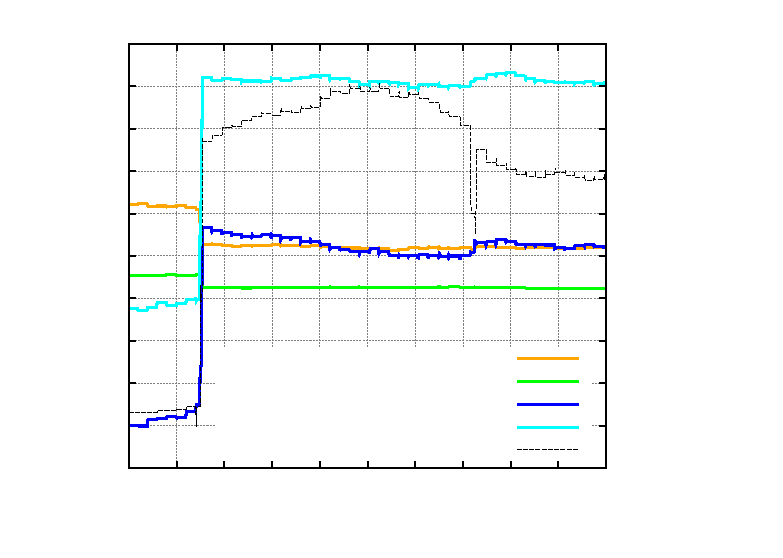
\includegraphics{eval_closeness}}%
    \gplfronttext
  \end{picture}%
\endgroup

%     \caption{Avg. Closeness Centrality of PolderCast and Scribe}
%     \label{fig:eval_closeness}
% \end{figure}

% \begin{figure}[H]
%     \centering
%     % GNUPLOT: LaTeX picture with Postscript
\begingroup
  \makeatletter
  \providecommand\color[2][]{%
    \GenericError{(gnuplot) \space\space\space\@spaces}{%
      Package color not loaded in conjunction with
      terminal option `colourtext'%
    }{See the gnuplot documentation for explanation.%
    }{Either use 'blacktext' in gnuplot or load the package
      color.sty in LaTeX.}%
    \renewcommand\color[2][]{}%
  }%
  \providecommand\includegraphics[2][]{%
    \GenericError{(gnuplot) \space\space\space\@spaces}{%
      Package graphicx or graphics not loaded%
    }{See the gnuplot documentation for explanation.%
    }{The gnuplot epslatex terminal needs graphicx.sty or graphics.sty.}%
    \renewcommand\includegraphics[2][]{}%
  }%
  \providecommand\rotatebox[2]{#2}%
  \@ifundefined{ifGPcolor}{%
    \newif\ifGPcolor
    \GPcolortrue
  }{}%
  \@ifundefined{ifGPblacktext}{%
    \newif\ifGPblacktext
    \GPblacktexttrue
  }{}%
  % define a \g@addto@macro without @ in the name:
  \let\gplgaddtomacro\g@addto@macro
  % define empty templates for all commands taking text:
  \gdef\gplbacktext{}%
  \gdef\gplfronttext{}%
  \makeatother
  \ifGPblacktext
    % no textcolor at all
    \def\colorrgb#1{}%
    \def\colorgray#1{}%
  \else
    % gray or color?
    \ifGPcolor
      \def\colorrgb#1{\color[rgb]{#1}}%
      \def\colorgray#1{\color[gray]{#1}}%
      \expandafter\def\csname LTw\endcsname{\color{white}}%
      \expandafter\def\csname LTb\endcsname{\color{black}}%
      \expandafter\def\csname LTa\endcsname{\color{black}}%
      \expandafter\def\csname LT0\endcsname{\color[rgb]{1,0,0}}%
      \expandafter\def\csname LT1\endcsname{\color[rgb]{0,1,0}}%
      \expandafter\def\csname LT2\endcsname{\color[rgb]{0,0,1}}%
      \expandafter\def\csname LT3\endcsname{\color[rgb]{1,0,1}}%
      \expandafter\def\csname LT4\endcsname{\color[rgb]{0,1,1}}%
      \expandafter\def\csname LT5\endcsname{\color[rgb]{1,1,0}}%
      \expandafter\def\csname LT6\endcsname{\color[rgb]{0,0,0}}%
      \expandafter\def\csname LT7\endcsname{\color[rgb]{1,0.3,0}}%
      \expandafter\def\csname LT8\endcsname{\color[rgb]{0.5,0.5,0.5}}%
    \else
      % gray
      \def\colorrgb#1{\color{black}}%
      \def\colorgray#1{\color[gray]{#1}}%
      \expandafter\def\csname LTw\endcsname{\color{white}}%
      \expandafter\def\csname LTb\endcsname{\color{black}}%
      \expandafter\def\csname LTa\endcsname{\color{black}}%
      \expandafter\def\csname LT0\endcsname{\color{black}}%
      \expandafter\def\csname LT1\endcsname{\color{black}}%
      \expandafter\def\csname LT2\endcsname{\color{black}}%
      \expandafter\def\csname LT3\endcsname{\color{black}}%
      \expandafter\def\csname LT4\endcsname{\color{black}}%
      \expandafter\def\csname LT5\endcsname{\color{black}}%
      \expandafter\def\csname LT6\endcsname{\color{black}}%
      \expandafter\def\csname LT7\endcsname{\color{black}}%
      \expandafter\def\csname LT8\endcsname{\color{black}}%
    \fi
  \fi
  \setlength{\unitlength}{0.0500bp}%
  \begin{picture}(7200.00,5040.00)%
    \gplgaddtomacro\gplbacktext{%
      \csname LTb\endcsname%
      \put(814,704){\makebox(0,0)[r]{\strut{} 0}}%
      \csname LTb\endcsname%
      \put(814,1111){\makebox(0,0)[r]{\strut{} 1}}%
      \csname LTb\endcsname%
      \put(814,1518){\makebox(0,0)[r]{\strut{} 2}}%
      \csname LTb\endcsname%
      \put(814,1925){\makebox(0,0)[r]{\strut{} 3}}%
      \csname LTb\endcsname%
      \put(814,2332){\makebox(0,0)[r]{\strut{} 4}}%
      \csname LTb\endcsname%
      \put(814,2740){\makebox(0,0)[r]{\strut{} 5}}%
      \csname LTb\endcsname%
      \put(814,3147){\makebox(0,0)[r]{\strut{} 6}}%
      \csname LTb\endcsname%
      \put(814,3554){\makebox(0,0)[r]{\strut{} 7}}%
      \csname LTb\endcsname%
      \put(814,3961){\makebox(0,0)[r]{\strut{} 8}}%
      \csname LTb\endcsname%
      \put(814,4368){\makebox(0,0)[r]{\strut{} 9}}%
      \csname LTb\endcsname%
      \put(814,4775){\makebox(0,0)[r]{\strut{} 10}}%
      \csname LTb\endcsname%
      \put(946,484){\makebox(0,0){\strut{} 0}}%
      \csname LTb\endcsname%
      \put(1417,484){\makebox(0,0){\strut{} 100}}%
      \csname LTb\endcsname%
      \put(1889,484){\makebox(0,0){\strut{} 200}}%
      \csname LTb\endcsname%
      \put(2360,484){\makebox(0,0){\strut{} 300}}%
      \csname LTb\endcsname%
      \put(2831,484){\makebox(0,0){\strut{} 400}}%
      \csname LTb\endcsname%
      \put(3303,484){\makebox(0,0){\strut{} 500}}%
      \csname LTb\endcsname%
      \put(3774,484){\makebox(0,0){\strut{} 600}}%
      \csname LTb\endcsname%
      \put(4245,484){\makebox(0,0){\strut{} 700}}%
      \csname LTb\endcsname%
      \put(4716,484){\makebox(0,0){\strut{} 800}}%
      \csname LTb\endcsname%
      \put(5188,484){\makebox(0,0){\strut{} 900}}%
      \csname LTb\endcsname%
      \put(5659,484){\makebox(0,0){\strut{} 1000}}%
      \put(5791,704){\makebox(0,0)[l]{\strut{} 0}}%
      \put(5791,1111){\makebox(0,0)[l]{\strut{} 100}}%
      \put(5791,1518){\makebox(0,0)[l]{\strut{} 200}}%
      \put(5791,1925){\makebox(0,0)[l]{\strut{} 300}}%
      \put(5791,2332){\makebox(0,0)[l]{\strut{} 400}}%
      \put(5791,2740){\makebox(0,0)[l]{\strut{} 500}}%
      \put(5791,3147){\makebox(0,0)[l]{\strut{} 600}}%
      \put(5791,3554){\makebox(0,0)[l]{\strut{} 700}}%
      \put(5791,3961){\makebox(0,0)[l]{\strut{} 800}}%
      \put(5791,4368){\makebox(0,0)[l]{\strut{} 900}}%
      \put(5791,4775){\makebox(0,0)[l]{\strut{} 1000}}%
      \put(176,2739){\rotatebox{-270}{\makebox(0,0){\strut{}Eccentricity Centrality}}}%
      \put(6692,2739){\rotatebox{-270}{\makebox(0,0){\strut{}Network Size}}}%
      \put(3302,154){\makebox(0,0){\strut{}Reporter Intervals}}%
    }%
    \gplgaddtomacro\gplfronttext{%
      \csname LTb\endcsname%
      \put(4672,1757){\makebox(0,0)[r]{\strut{}PolderCast (Facebook)}}%
      \csname LTb\endcsname%
      \put(4672,1537){\makebox(0,0)[r]{\strut{}PolderCast (Twitter)}}%
      \csname LTb\endcsname%
      \put(4672,1317){\makebox(0,0)[r]{\strut{}Scribe (Facebook)}}%
      \csname LTb\endcsname%
      \put(4672,1097){\makebox(0,0)[r]{\strut{}Scribe (Twitter)}}%
      \csname LTb\endcsname%
      \put(4672,877){\makebox(0,0)[r]{\strut{}Network Size}}%
    }%
    \gplbacktext
    \put(0,0){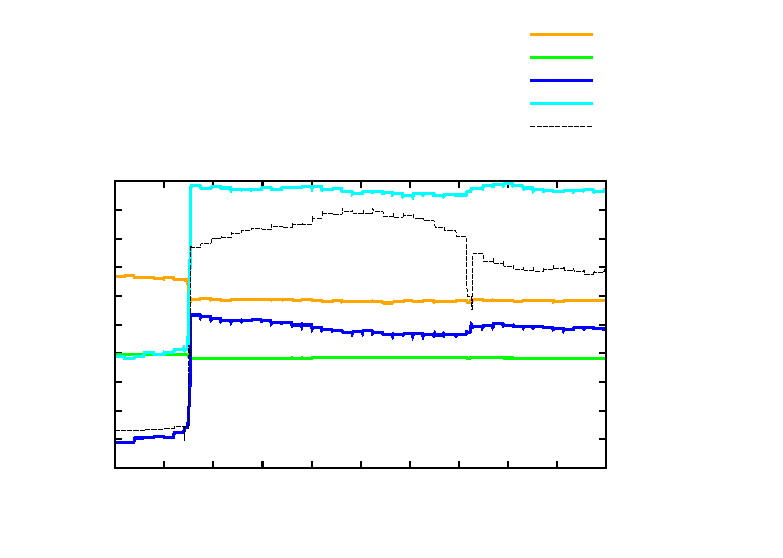
\includegraphics{eval_eccentricity}}%
    \gplfronttext
  \end{picture}%
\endgroup

%     \caption{Avg. Eccentricity Centrality of PolderCast and Scribe}
%     \label{fig:eval_eccentricity}
% \end{figure}

